\documentclass[crop,tikz]{standalone}
\usetikzlibrary{backgrounds}
\colorlet{blue}{cyan}
\tikzset{
  inverted/.style = {
    every path/.style = {draw=white,text=white},
    background rectangle/.style={fill},
    show background rectangle
  }
}

\begin{document}
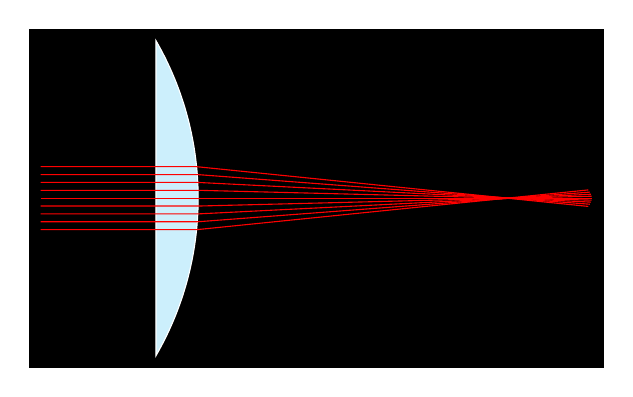
\begin{tikzpicture}[inverted,inverted]
  \pgfmathsetmacro{\radius}{4}
  \pgfmathsetmacro{\refractiveindex}{2}
  \draw[fill=cyan!20] (-30:\radius) arc (-30:30:\radius) -- cycle;
  \foreach \Y in { -0.4,-0.3,...,0.4 } {%
    \pgfmathsetmacro{\X}{sqrt(\radius*\radius-\Y*\Y)}
    \pgfmathsetmacro{\angle}{atan(\Y/\X)}
    \draw[red] (2, \Y) -- ({\X}, \Y) -- +({\angle - asin(\refractiveindex*sin(\angle))}:5);
  }
\end{tikzpicture}
\end{document}
